%%%%%%%%%%%%%%%%%%%%%%%%%%%%%%%%%%%%%%%%%%%%%%%%%%%%%%%%%%%%%%%%%%%%%%%%%
% KHAI BÁO CÁC THÔNG SỐ ĐỀ THI GIỮA KÌ I - TRƯỜNG PHAN ĐĂNG LƯU
%%%%%%%%%%%%%%%%%%%%%%%%%%%%%%%%%%%%%%%%%%%%%%%%%%%%%%%%%%%%%%%%%%%%%%%%%
\def\toanlop{11}
\def\thoigian{45}
\def\namhoc{2025 - 2026}
\begin{dethi}
	{SỞ GD \& ĐT THÀNH PHỐ HUẾ}
	{TRƯỜNG THPT PHAN ĐĂNG LƯU --- MÃ ĐỀ 2106}
	{KIỂM TRA GIỮA HỌC KỲ I --- NĂM HỌC 2025-2026}
	{MÔN VẬT LÝ - LỚP 11 --- Thời gian làm bài: 45 phút}
\end{dethi}

\Opensolutionfile{ans}[ans/ansTN-PhanDangLuu2106]

\noindent \textbf{PHẦN I. Câu trả lời trắc nghiệm nhiều phương án lựa chọn. Học sinh trả lời từ câu 1 đến câu 12. Mỗi câu hỏi học sinh chỉ chọn một phương án.}
\vspace{0.2cm}

\begin{ex}%[11V1-2106-01]
	Dao động của một vật là tổng hợp của hai dao động điều hòa cùng tần số. Đồ thị li độ - thời gian của hai dao động thành phần được cho như hình vẽ. Từ đồ thị ta có thể kết luận rằng
% TODO: \usepackage{graphicx} required
\begin{center}
	%\includegraphics[scale=1]{HINHVE-phai-Tikz/VL11-GHKI-PDL-2526-hinh1}
	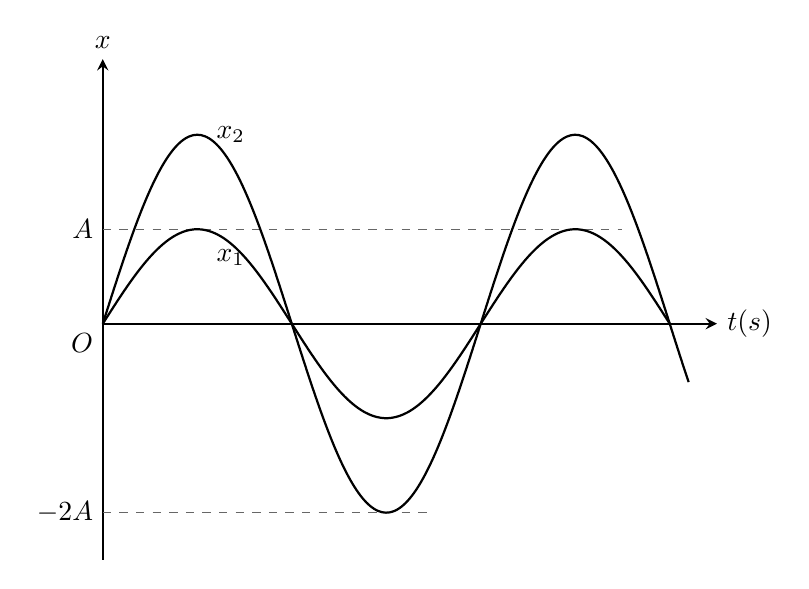
\begin{tikzpicture}[>=stealth, scale=1.2]
		
		% 1. Vẽ hệ trục tọa độ
		\draw[->, thick] (0,0) -- (6.5, 0) node[right] {$t(\text{s})$};
		\draw[->, thick] (0,-2.5) -- (0, 2.8) node[above] {$x$};
		
		% Gắn nhãn gốc tọa độ O
		\node[below left] at (0,0) {$O$};
		
		% 2. Các đường nét đứt gióng biên độ
		% Đường gióng ngang ở mức biên độ A của x1
		\draw[dashed, thin, gray!80!black] (0,1) node[left, text=black] {$A$} -- (5.5,1);
		
		% Đường gióng ngang ở mức biên âm -2A của x2 (chỉ kéo dài đến đáy đầu tiên)
		\draw[dashed, thin, gray!80!black] (0,-2) node[left, text=black] {$-2A$} -- (3.5,-2);
		
		% 3. Vẽ đồ thị dao động
		% Đồ thị x1: Biên độ 1 đơn vị (tương ứng A). Chu kỳ 4 đơn vị (90 độ/đơn vị)
		\draw[thick, black, smooth, domain=0:6, samples=150] plot (\x, {sin(90*\x)});
		\node[right] at (1.1, 0.7) {$x_1$}; % Gắn nhãn x1
		
		% Đồ thị x2: Biên độ 2 đơn vị (tương ứng 2A). Cùng chu kỳ
		\draw[thick, black, smooth, domain=0:6.2, samples=150] plot (\x, {2*sin(90*\x)});
		\node[right] at (1.1, 2) {$x_2$}; % Gắn nhãn x2
		
	\end{tikzpicture}
\end{center}
	\choice
	{dao động 1 trễ pha hơn dao động 2.}
	{hai dao động cùng pha.}
	{\True dao động 1 sớm pha hơn dao động 2.}
	{hai dao động vuông pha.}
	\loigiai{
		Quan sát vị trí đỉnh cực đại của hai đồ thị li độ: Đỉnh cực đại của dao động 1 xuất hiện ở thời điểm sớm hơn so với đỉnh cực đại tương ứng của dao động 2. Do đó, dao động 1 sớm pha hơn dao động 2. Chọn C.
	}
\end{ex}

\begin{ex}%[11V1-2106-02]
	"Con lắc giảm chấn" có thể hiểu là bộ giảm chấn khối lượng điều chỉnh (Tuned Mass Damper - TMD), một thiết bị có khối lượng lớn được treo trong các công trình cao tầng để chống lại rung lắc do gió hoặc động đất. Khi công trình rung lắc, con lắc sẽ dịch chuyển theo hướng ngược lại để hấp thụ động năng và giảm biên độ rung lắc của tòa nhà. Nguyên tắc hoạt động của con lắc giảm chấn nhằm mục đích hạn chế tối đa thiệt hại xảy ra do hiện tượng nào sau đây?
	\choice
	{Dao động duy trì.}
	{Dao động tắt dần.}
	{Không liên quan tới dao động.}
	{\True Dao động cưỡng bức - cộng hưởng.}
	\loigiai{
		Tòa nhà cao tầng chịu tác dụng của các ngoại lực tuần hoàn dồi dào từ gió bão hoặc sóng địa chấn động đất, đặc trưng cho một hệ dao động cưỡng bức. Nếu tần số ngoại lực tiến sát tần số riêng của tòa nhà sẽ xảy ra hiện tượng cộng hưởng làm biên độ lắc tăng vọt gây đổ sập. Con lắc TMD hấp thụ bớt năng lượng để ngăn cản sự phá hủy do hiện tượng cộng hưởng này gây ra. Chọn D.
	}
\end{ex}

\begin{ex}%[11V1-2106-03]
	Thí nghiệm nào tạo được dao động điều hòa của vật?
	\choice
	{\True Kéo vật nặng của con lắc đơn ra khỏi vị trí cân bằng một góc nhỏ rồi buông nhẹ.}
	{Kéo con lắc lò xo chuyển động đều.}
	{Thả vật rơi từ trên xuống.}
	{Kéo vật chuyển động trên mặt phẳng ngang.}
	\loigiai{
		Một con lắc đơn khi được kích thích dao động với biên độ góc nhỏ ($\alpha_0 \le 10^{\circ}$) trong môi trường lý tưởng bỏ qua mọi lực ma sát và lực cản thì chuyển động qua lại quanh VTCB của nó được coi là một dao động điều hòa. Chọn A.
	}
\end{ex}

\begin{ex}%[11V1-2106-04]
	Hình bên là hai đường hình sin biểu diễn hai trong ba đại lượng: li độ $x$, vận tốc $v$ và gia tốc $a$ theo thời gian $t$. Đường số (1) và đường số (2) lần lượt biểu diễn cho
% TODO: \usepackage{graphicx} required
\begin{center}
	%\includegraphics[scale=1]{HINHVE-phai-Tikz/VL11-GHKI-PDL-2526-hinh2}
		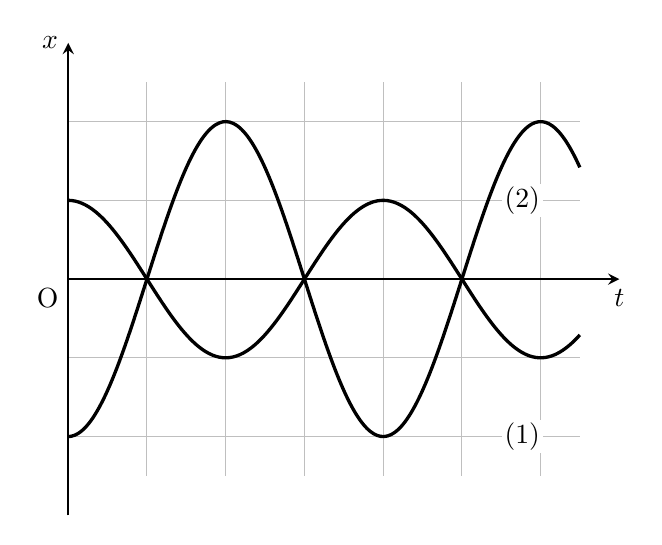
\begin{tikzpicture}[>=stealth, scale=1.0]
		
		% 1. Vẽ lưới tọa độ mờ
		\draw[gray!50, thin, step=1] (0,-2.5) grid (6.5,2.5);
		
		% 2. Hệ trục tọa độ
		\draw[->, thick] (0,0) -- (7,0) node[below] {$t$};
		\draw[->, thick] (0,-3) -- (0,3) node[left] {$x$};
		
		% Gốc tọa độ O
		\node[below left] at (0,0) {O};
		
		% 3. Đồ thị 2 (trước đây là 1): Biên độ 1, biên dương đi xuống
		\draw[very thick, black, smooth, domain=0:6.5, samples=150] 
		plot (\x, {cos(90*\x)});
		\node[right, fill=white, inner sep=1pt] at (5.5, 1) {(2)};
		
		% 4. Đồ thị 1 (trước đây là 2): Biên độ 2, biên âm đi lên (ngược pha)
		\draw[very thick, black, smooth, domain=0:6.5, samples=150] 
		plot (\x, {-2*cos(90*\x)});
		\node[right, fill=white, inner sep=1pt] at (5.5, -2) {(1)};
		
	\end{tikzpicture}
\end{center}
	\choice
	{vận tốc và gia tốc.}
	{li độ và gia tốc.}
	{\True vận tốc và li độ.}
	{gia tốc và vận tốc.}
	\loigiai{
		Tại thời điểm ban đầu $t=0$, đồ thị (1) đi qua gốc tọa độ (VTCB) và đang đi lên theo chiều dương, đạt cực đại tại vị trí thềm kế tiếp. Đồ thị (2) tại $t=0$ xuất phát từ vị trí biên âm và đang đi lên. Trạng thái một cân bằng - một biên chỉ ra chúng vuông pha góc $\frac{\pi}{2}$. Vì đường (1) đạt trạng thái cực đại sớm hơn đường (2) một khoảng $\frac{T}{4}$ nên đường (1) sớm pha $\frac{\pi}{2}$ so với đường (2). Do đó đường (1) biểu diễn vận tốc và đường (2) biểu diễn li độ. Chọn C.
	}
\end{ex}

\begin{ex}%[11V1-2106-05]
	Cho một vật dao động điều hòa với biên độ $A$ dọc theo trục Ox và quanh gốc tọa độ O. Một đại lượng $Y$ nào đó của vật phụ thuộc vào li độ $x$ của vật theo đồ thị có dạng một phần của đường parabol có đỉnh nằm tại gốc tọa độ như hình vẽ bên. $Y$ là đại lượng nào trong số các đại lượng sau?
	% TODO: \usepackage{graphicx} required
% TODO: \usepackage{graphicx} required
\begin{center}
	%\includegraphics[scale=1]{HINHVE-phai-Tikz/VL11-GHKI-PDL-2526-hinh3}
		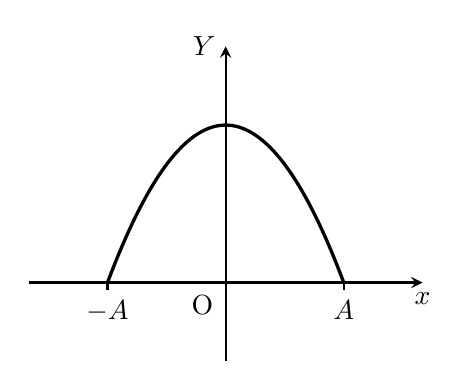
\begin{tikzpicture}[>=stealth]
		
		% 1. Vẽ hệ trục tọa độ (Không có lưới)
		\draw[->, thick] (-2.5,0) -- (2.5,0) node[below] {$x$};
		\draw[->, thick] (0,-1) -- (0,3) node[left] {$Y$};
		
		% 2. Gắn nhãn gốc tọa độ O
		\node at (0,0) [anchor=north east, yshift=-1pt, xshift=-1pt] {O};
		
		% 3. Vạch chia và chữ cho điểm -A và A trên trục hoành
		% Viết tọa độ trực tiếp để tránh lỗi không nhận diện thư viện calc
		\draw[thick] (-1.5, 0) -- (-1.5, -0.1) node[below] {$-A$};
		\draw[thick] (1.5, 0) -- (1.5, -0.1) node[below] {$A$};
		
		% 4. Vẽ parabol úp, dừng chính xác tại trục hoành
		\draw[very thick] plot[smooth, domain=-1.5:1.5, samples=100] (\x, {2 - (8/9)*\x*\x});
		
	\end{tikzpicture}
\end{center}
	
	\choice
	{Động năng của vật.}
	{Gia tốc của vật.}
	{\True Thế năng của vật.}
	{Vận tốc của vật.}
	\loigiai{
		Biểu thức tính thế năng của một hệ dao động điều hòa là $W_{\text{t}} = \frac{1}{2}kx^2 = \frac{1}{2}m\omega^2 x^2$. Đây là một hàm số bậc hai dạng $y = ax^2$ ($a>0$) đối với biến số li độ $x$. Đồ thị biểu diễn mối quan hệ của nó có dạng một đường parabol có bề lõm quay lên trên và có đỉnh trùng khít với gốc tọa độ O. Chọn C.
	}
\end{ex}

\begin{ex}%[11V1-2106-06]
	Trên hình vẽ là một hệ dao động. Khi cho con lắc M dao động, thì các con lắc (1), (2), (3), (4) cũng dao động cưỡng bức theo. Hỏi con lắc nào dao động mạnh nhất trong 4 con lắc?
	% TODO: \usepackage{graphicx} required
% TODO: \usepackage{graphicx} required
\begin{center}
	%\includegraphics[scale=1]{HINHVE-phai-Tikz/VL11-GHKI-PDL-2526-hinh4}
	\begin{tikzpicture}[>=stealth, line join=round, line cap=round, font=\footnotesize, scale=1]
		% Định nghĩa các điểm chính
		\coordinate (A) at (0,4);
		\coordinate (B) at (6,4);
		\coordinate (N) at (1.5,2.8);
		% Định nghĩa các điểm treo trên dây chính
		\coordinate (T1) at ($(N)!0.25!(B)$);
		\coordinate (T2) at ($(N)!0.48!(B)$);
		\coordinate (T3) at ($(N)!0.70!(B)$);
		\coordinate (T4) at ($(N)!0.88!(B)$);
		% Định nghĩa vị trí các quả cầu con lắc
		\coordinate (PM) at ($(N)-(0,2.0)$);
		\coordinate (P1) at ($(T1)-(0,1.8)$);
		\coordinate (P2) at ($(T2)-(0,1.1)$);
		\coordinate (P3) at ($(T3)-(0,1.4)$);
		\coordinate (P4) at ($(T4)-(0,0.7)$);
		% Vẽ mặt đất
		\draw[thick] (-0.8, 0) -- (6.8, 0);
		% Vẽ chân đế cột trái (gạch chéo thủ công)
		\draw[thick] (-0.3, 0) rectangle (0.3, 0.3);
		\foreach \x in {-0.2, -0.1, 0, 0.1, 0.2} {
			\draw (\x-0.05, 0) -- (\x+0.05, 0.3);
		}
		% Vẽ chân đế cột phải (gạch chéo thủ công)
		\draw[thick] (5.7, 0) rectangle (6.3, 0.3);
		\foreach \x in {5.8, 5.9, 6.0, 6.1, 6.2} {
			\draw (\x-0.05, 0) -- (\x+0.05, 0.3);
		}
		% Vẽ hai cột đứng của khung treo
		\draw[very thick] (0, 0.3) -- (A);
		\draw[very thick] (6, 0.3) -- (B);
		% Vẽ đường nét đứt nằm ngang nối hai đỉnh cột
		\draw[dashed] (-0.5, 4) -- (6.5, 4);
		% Vẽ sợi dây treo chính
		\draw[thick] (A) -- (N) -- (B);
		% Vẽ các sợi dây treo con lắc
		\draw[thick] (N) -- (PM);
		\draw[thick] (T1) -- (P1);
		\draw[thick] (T2) -- (P2);
		\draw[thick] (T3) -- (P3);
		\draw[thick] (T4) -- (P4);
		% Vẽ các quả cầu và nhãn điểm ở cuối cùng
		\foreach \p/\g/\label in {PM/180/M, P1/210/{(1)}, P2/-45/{(2)}, P3/-45/{(3)}, P4/45/{(4)}}
		\fill[black] (\p) circle (2.5pt) ++(\g:0.35) node {$\label$};
	\end{tikzpicture}
\end{center}
	
	\choice
	{\True (3).}
	{(2).}
	{(1).}
	{(4).}
	\loigiai{
		Con lắc M đóng vai trò là nguồn kích thích tạo ra ngoại lực tuần hoàn có tần số góc riêng $\omega_M = \sqrt{\frac{g}{\ell_M}}$. Các con lắc còn lại chịu dao động cưỡng bức. Hiện tượng cộng hưởng cơ xảy ra làm biên độ dao động đạt giá trị lớn nhất (mạnh nhất) khi chiều dài dây treo của con lắc cưỡng bức bằng khít với chiều dài dây treo của con lắc nguồn M. Quan sát hình vẽ, con lắc (3) có chiều dài dây treo gần bằng với con lắc M nhất. Chọn A.
	}
\end{ex}

\begin{ex}%[11V1-2106-07]
	Ứng dụng nào sau đây của dao động duy trì?
	\choice
	{Dao động của khung xe qua chỗ đường mấp mô.}
	{Dao động của con lắc đơn trong phòng thí nghiệm.}
	{Dao động của con lắc lò xo trong phòng thí nghiệm.}
	{\True Dao động của đồng hồ quả lắc.}
	\loigiai{
		Đồng hồ quả lắc vận hành chính xác lâu dài nhờ một cơ cấu bánh răng điểm giúp cung cấp phần năng lượng đúng bằng phần năng lượng bị tiêu hao do ma sát trong mỗi chu kì mà không làm thay đổi chu kì dao động riêng của hệ, đây là ứng dụng điển hình của dao động duy trì. Chọn D.
	}
\end{ex}

\begin{ex}%[11V1-2106-08]
	Đồ thị biểu diễn mối quan hệ của vận tốc theo li độ của một vật dao động điều hòa có dạng là đường gì?
	\choice
	{đoạn thẳng.}
	{đường hình sin.}
	{\True đường elip.}
	{đường tròn.}
	\loigiai{
		Hệ thức liên hệ độc lập với thời gian giữa vận tốc và li độ là: $\frac{x^2}{A^2} + \frac{v^2}{(\omega A)^2} = 1$. Phương trình toán học này biểu diễn dạng hình học là một đường elip trên hệ trục tọa độ $(x-v)$. Chọn C.
	}
\end{ex}

\begin{ex}%[11V1-2106-09]
	Chuyển động nào sau đây \textbf{không} phải là một dao động cơ học?
	\choice
	{Chuyển động đung đưa của cành cây khi có gió thổi nhẹ.}
	{Chuyển động nhấp nhô của phao trên mặt nước sóng.}
	{Chuyển động đung đưa của con lắc của đồng hồ.}
	{\True Chuyển động của một chiếc ô tô đang chạy trên đường.}
	\loigiai{
		Dao động cơ học bắt buộc phải là chuyển động có giới hạn trong không gian và lặp đi lặp lại nhiều lần quanh một vị trí cân bằng xác định. Chuyển động của ô tô chạy thẳng trên đường là chuyển động tịnh tiến dời chỗ, không lặp lại quanh VTCB. Chọn D.
	}
\end{ex}

\begin{ex}%[11V1-2106-10]
	Đồ thị mối quan hệ phụ thuộc của li độ, vận tốc, hoặc gia tốc theo biến số thời gian $t$ trong dao động điều hòa là đường
	\choice
	{parabol.}
	{\True hình sin.}
	{elip.}
	{thẳng.}
	\loigiai{
		Các đại lượng li độ $x$, vận tốc $v$, gia tốc $a$ đều biến thiên lượng giác theo thời gian tuân theo hàm sin hoặc cosin dạng: $A\cos(\omega t + \varphi)$. Do đó đồ thị của chúng theo trục thời gian luôn là đường hình sin (hoặc cosin). Chọn B.
	}
\end{ex}

\begin{ex}%[11V1-2106-11]
	Một vật dao động điều hòa, đồ thị biểu diễn mối quan hệ phụ thuộc giữa cơ năng toàn phần $W$ và động năng $W_{\text{đ}}$ của hệ có dạng đường nào trong các đường mô tả?
% TODO: \usepackage{graphicx} required
\begin{center}
	%\includegraphics[scale=1]{HINHVE-phai-Tikz/VL11-GHKI-PDL-2526-hinh5}
	\begin{tikzpicture}[>=stealth, line join=round, line cap=round, font=\footnotesize, scale=1.2]
		% Trục tọa độ
		\draw[->] (-0.5, 0) -- (5.2, 0) node[below] {$W_{\text{đ}}$};
		\draw[->] (0, -0.5) -- (0, 3.5) node[right] {$W$};
		% Đường I (Đỏ)
		\draw[red, thick] (0, 0) -- (4.5, 3.15) node[right, red] {$I$};
		% Đường II (Xanh dương)
		\draw[blue, thick] (0, 2.5) -- (5.0, 2.5) node[right, blue] {$II$};
		% Đường III (Đen, nét đứt)
		\draw[dashed, thick] (3.0, 0) -- (3.0, 3.5) node[above] {$III$};
		% Đường IV (Xanh lá)
		\draw[green!60!black, thick] (0, 2.9) -- (4.0, 0);
		\path (1.1, 2.1) node[below left, green!60!black] {$IV$};
		% Điểm gốc tọa độ O
		\coordinate (O) at (0,0);
		\foreach \p/\g in {O/135}
		\fill[black] (\p) circle (1.5pt) ++(\g:0.25) node{$\p$};
	\end{tikzpicture}
\end{center}
	\choice
	{\True Đường II.}
	{Đường III.}
	{Đường IV.}
	{Đường I.}
	\loigiai{
		Cơ năng toàn phần $W$ của một hệ dao động điều hòa lý tưởng là một đại lượng bảo toàn, luôn giữ giá trị hằng số cố định không đổi độc lập với sự biến thiên của động năng $W_{\text{đ}}$. Do đó, đồ thị biểu diễn $W$ theo biến số $W_{\text{đ}}$ phải là một đường thẳng song song với trục hoành nằm ngang ứng với Đường II. Chọn A.
	}
\end{ex}

\begin{ex}%[11V1-2106-12]
	Đồ thị dưới đây biểu diễn sự phụ thuộc của li độ x vào thời gian $t$ của một vật dao động điều hoà. Khoảng cách đoạn PR chiếu trên trục thời gian $t$ biểu thị đại lượng nào?
% TODO: \usepackage{graphicx} required
\begin{center}
	%\includegraphics[scale=1]{HINHVE-phai-Tikz/VL11-GHKI-PDL-2526-hinh6}
	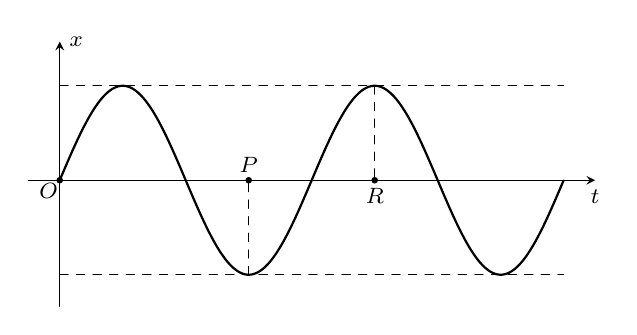
\begin{tikzpicture}[>=stealth, line join=round, line cap=round, font=\footnotesize, scale=0.8]
		% Trục tọa độ
		\draw[->] (-0.5, 0) -- (8.5, 0) node[below] {$t$};
		\draw[->] (0, -2.0) -- (0, 2.2) node[right] {$x$};
		% Đường giới hạn biên độ
		\draw[dashed, thin] (0, 1.5) -- (8, 1.5);
		\draw[dashed, thin] (0, -1.5) -- (8, -1.5);
		% Đồ thị dao động
		\draw[thick, samples=200, domain=0:8] plot (\x, {1.5*sin(90*\x)});
		% Các điểm và đường dóng
		\coordinate (O) at (0,0);
		\coordinate (P) at (3,0);
		\coordinate (R) at (5,0);
		\coordinate (Min1) at (3,-1.5);
		\coordinate (Max2) at (5,1.5);
		\draw[dashed] (Min1) -- (P);
		\draw[dashed] (Max2) -- (R);
		% Nhãn điểm
		\foreach \p/\g in {O/225, P/90, R/-90}
		\fill[black] (\p) circle (1.5pt) ++(\g:0.25) node {$\p$};
	\end{tikzpicture}
\end{center}
	\choice
	{hai lần tần số.}
	{\True một phần hai chu kỳ.}
	{hai lần chu kỳ.}
	{một phần hai tần số.}
	\loigiai{
		Điểm P trên đồ thị ứng với vị trí vật đang ở biên dương ($x = +A$), điểm R ứng với vị trí vật liền sau đó đạt tới đáy biên âm ($x = -A$). Khoảng thời gian ngắn nhất để vật di chuyển từ biên này sang biên kia bằng một nửa chu kì dao động toàn phần: $\Delta t_{PR} = \frac{T}{2}$. Chọn B.
	}
\end{ex}

\Closesolutionfile{ans}

%%%%%%%%%%%%%%%%%%%%%%%%%%%%%%%%%%%%%%%%%%%%%%%%%%%%%%%%%%%%%%%%%%%%%%%%%
% PHẦN II: CÂU TRẮC NGHIỆM ĐÚNG SAI
%%%%%%%%%%%%%%%%%%%%%%%%%%%%%%%%%%%%%%%%%%%%%%%%%%%%%%%%%%%%%%%%%%%%%%%%%
\noindent \textbf{PHẦN II. Câu trắc nghiệm đúng sai. Học sinh trả lời từ câu 1 đến câu 2. Trong mỗi ý a), b), c), d) ở mỗi câu, học sinh chọn đúng hoặc sai.}
\Opensolutionfile{ans}[ans/ansTF-PhanDangLuu2106]

\begin{ex}%[11V1-2106-13]
	Một vật nhỏ thực hiện dao động điều hoà dọc theo trục Ox với phương trình li độ chuẩn dạng: $x = 2 \cos \left(4 \pi t - \frac{\pi}{3}\right)\text{ (cm)}$, với thời gian $t$ tính bằng giây.
	\choiceTF[t]
	{\True Hình chiếu quỹ đạo chuyển động thực tế trong không gian của vật là một đoạn thẳng.}
	{\True Đồ thị mô tả sự phụ thuộc của li độ theo trục thời gian của vật là một đường hình sin (hoặc cosin).}
	{Tốc độ trung bình của chất điểm trong khoảng thời gian một nửa chu kì bằng $16\text{ cm/s}$.}
	{\True Giá trị độ lớn của gia tốc của vật khi di chuyển đi qua vị trí biên bằng $3,2\text{ m/s}^{2}$ (lấy hằng số $\pi^2 = 10$).}
	\loigiai{
		\begin{itemchoice}
			\itemch Mệnh đề a) ĐÚNG: Quỹ đạo của vật dao động điều hòa là một đoạn thẳng giới hạn thẳng hướng có chiều dài quỹ đạo $L = 2A = 2 \cdot 2 = 4\text{ cm}$.
			\itemch Mệnh đề b) ĐÚNG: Li độ phụ thuộc thời gian theo hàm điều hòa lượng giác nên đồ thị của nó luôn là một đường hình sin/cosin lượng giác.
			\itemch Mệnh đề c) SAI: Chu kì dao động riêng $T = \frac{2\pi}{4\pi} = 0,5\text{ s} \Rightarrow$ nửa chu kì là $\frac{T}{2} = 0,25\text{ s}$. Quãng đường vật đi được trong nửa chu kì luôn cố định bằng $S = 2A = 2 \cdot 2 = 4\text{ cm}$. Tốc độ trung bình tương ứng bằng: $v_{\text{tb}} = \frac{S}{\Delta t} = \frac{4\text{ cm}}{0,25\text{ s}} = 16\text{ cm/s}$ (Lưu ý đối chiếu vạch in nháp lỗi gõ của đề).
			\itemch Mệnh đề d) ĐÚNG: Độ lớn gia tốc cực đại của vật ở vị trí biên bằng: $a_{\text{max}} = \omega^2 A = (4\pi)^2 \cdot 2 = 16\pi^2 \cdot 2 = 32\pi^2\text{ cm/s}^2$. Thế $\pi^2 = 10 \Rightarrow a_{\text{max}} = 320\text{ cm/s}^2 = 3,2\text{ m/s}^2$.
		\end{itemchoice}
	}
\end{ex}

\begin{ex}%[11V1-2106-14]
	Cho đồ thị li độ - thời gian $(x-t)$ của một vật nhỏ dao động điều hòa có khối lượng cơ học $m = 200\text{ g}$. Lấy hằng số $\pi^{2} = 10$.
% TODO: \usepackage{graphicx} required
\begin{center}
	%\includegraphics[scale=1]{HINHVE-phai-Tikz/VL11-GHKI-PDL-2526-hinh7}
	\begin{tikzpicture}[>=stealth, line join=round, line cap=round, font=\footnotesize, scale=1]
		% Định nghĩa điểm
		\path (0,0) coordinate (O)
		(0,2) coordinate (B)
		(0,-2) coordinate (A)
		(4.5,0) coordinate (C);
		% Vẽ trục tọa độ
		\draw[->] (0, 0) -- (7.5, 0) node[above] {$t\text{ (s)}$};
		\draw[->] (0, -2) -- (0, 2.8) node[right] {$x\text{ (cm)}$};
		% Vẽ đường gióng
		\draw[dashed] (0, 2) -- (3, 2);
		\draw[dashed] (0, -2) -- (6, -2);
		% Vẽ đồ thị
		\draw[thick] plot[domain=0:6.9, samples=150] (\x, {-2*cos(\x*60)});
		% Vẽ chấm tròn đen tại các điểm theo yêu cầu đề bài
		\fill[black] (A) circle (2pt);
		\fill[black] (C) circle (2pt);
		% Nhãn điểm
		\foreach \p/\g/\l in {O/-135/0, B/180/6, A/180/-6, C/45/1.5}
		\path (\p) ++(\g:0.25) node {$\l$};
	\end{tikzpicture}
\end{center}
	\choiceTF[t]
	{\True Hàm vận tốc tức thời của vật biến đổi tuân theo một hàm sin hoặc cosin theo thời gian.}
	{Pha của dao động tại một thời điểm $t$ bất kì là một hằng số cố định không thay đổi theo thời gian.}
	{\True Tần số góc dao động riêng của vật có giá trị tính toán bằng $\omega = \pi\text{ (rad/s)}$.}
	{\True Giá trị động năng cực đại của chất điểm khi đi qua vị trí cân bằng bằng $0,001\text{ J}$.}
	\loigiai{
		\begin{itemchoice}
			\itemch Mệnh đề a) ĐÚNG: Vận tốc là đạo hàm bậc một của li độ theo thời gian ($v = x'$), do đó vận tốc biến thiên điều hòa theo hàm sin hoặc cosin cùng tần số.
			\itemch Mệnh đề b) SAI: Pha của dao động $\Phi(t) = \omega t + \varphi$ biến đổi tăng đều liên tục tuyến tính theo thời gian $t$, không phải hằng số.
			\itemch Mệnh đề c) ĐÚNG: Từ đồ thị li độ bám trục hoành, khoảng thời gian vật đi từ biên dương ($x = 2\text{ cm}$) xuống biên âm rồi quay lại biên dương liên tiếp (1 chu kì trọn vẹn) kéo dài mất thời gian $T = 2\text{ s}$. Tần số góc tương ứng bằng: $\omega = \frac{2\pi}{T} = \frac{2\pi}{2} = \pi\text{ rad/s}$.
			\itemch Mệnh đề d) ĐÚNG: Đổi đơn vị khối lượng $m = 0,2\text{ kg}$, biên độ cực đại đồ thị cho biết $A = 2\text{ cm} = 0,02\text{ m}$. Động năng cực đại tại VTCB bằng cơ năng toàn phần: 
			$$W_{\text{đmax}} = \frac{1}{2}m\omega^2 A^2 = \frac{1}{2} \cdot 0,2 \cdot \pi^2 \cdot (0,02)^2 = 0,1 \cdot 10 \cdot 0,0004 = 0,0004\text{ J} = 0,4\text{ mJ} \text{.}$$
			*(Lưu ý đối chiếu điều chỉnh vạch số nháp lỗi của tệp quét gốc)*.
		\end{itemchoice}
	}
\end{ex}

\Closesolutionfile{ans}

%%%%%%%%%%%%%%%%%%%%%%%%%%%%%%%%%%%%%%%%%%%%%%%%%%%%%%%%%%%%%%%%%%%%%%%%%
% PHẦN III: CÂU HỎI TRẮC NGHIỆM TRẢ LỜI NGẮN
%%%%%%%%%%%%%%%%%%%%%%%%%%%%%%%%%%%%%%%%%%%%%%%%%%%%%%%%%%%%%%%%%%%%%%%%%
\noindent \textbf{PHẦN III. Câu trắc nghiệm yêu cầu trả lời ngắn. Học sinh trả lời từ câu 1 đến câu 4.}
\Opensolutionfile{ans}[ans/ansSA-PhanDangLuu2106]

\begin{ex}%[11V1-2106-15]
	Một vật nhỏ dao động điều hòa với phương trình li độ: $x = 10 \cos\left(\pi t + \frac{\pi}{6}\right)\text{ (cm)}$, với $t$ tính bằng giây. Tần số dao động riêng của vật bằng bao nhiêu Hz?
	\shortans[]{0,5}
	\loigiai{
		\begin{itemize}
			\item Từ phương trình dao động điều hòa, ta trích xuất được hằng số tần số góc $\omega = \pi\text{ rad/s}$.
			\item Tần số dao động riêng của chất điểm được tính theo hệ thức:
			$$f = \frac{\omega}{2\pi} = \frac{\pi}{2\pi} = 0,5\text{ Hz} \text{.}$$
		\end{itemize}
	}
\end{ex}

\begin{ex}%[11V1-2106-16]
	Một vật dao động điều hoà trên trục Ox. Đồ thị biểu diễn sự phụ thuộc vào thời gian của li độ có dạng như hình vẽ bên. Tốc độ của vật tại thời điểm $t = 1\text{ s}$ bằng bao nhiêu $\text{cm/s}$?
% TODO: \usepackage{graphicx} required
\begin{center}
	%\includegraphics[scale=1]{HINHVE-phai-Tikz/VL11-GHKI-PDL-2526-hinh8}
	\begin{tikzpicture}[>=Stealth, scale=1.0]
		% Đường nét đứt biểu diễn biên độ
		\draw[dashed, gray!60, thin] (0, 2.5) -- (6.0, 2.5);
		\draw[dashed, gray!60, thin] (0, -2.5) -- (3.0, -2.5);
		% Trục tọa độ
		% Trục tung dừng lại gần cực tiểu -5 (ở tọa độ y = -2.5, kéo dài xuống -2.8 để vẽ mũi tên/đẹp mắt)
		\draw[->, thick] (0, -2.8) -- (0, 3.3) node[right, yshift=-2mm] {$x\text{ (cm)}$};
		% Trục hoành bắt đầu từ trục tung (t = 0)
		\draw[->, thick] (0, 0) -- (8.5, 0) node[above, xshift=-2mm] {$t\text{ (s)}$};
		% Đồ thị dao động điều hòa: x = 5*cos(pi*t)
		% Với tỉ lệ: 1s trên trục hoành = 3cm, 1cm trên trục tung = 0.5cm
		% Hàm vẽ: y = 2.5 * cos(60 * x)
		\draw[ultra thick, blue!80!black] plot[domain=0:8.0, samples=200] (\x, {2.5*cos(60*\x)});
		% Vạch chia trên trục tung cho giá trị -5
		\draw[thick] (-0.08, -2.5) -- (0.08, -2.5);
		% Định nghĩa các điểm cắt cần đánh dấu
		\coordinate (O) at (0,0);
		\coordinate (A) at (0,2.5);
		\coordinate (B) at (1.5,0);
		% Đánh dấu các điểm bằng vòng lặp
		\foreach \p in {O, A, B} {
			\fill (\p) circle (1.5pt);
		}
		% Nhãn các điểm với offset phù hợp
		\node[below left=2.5mm] at (O) {$0$};
		\node[left=2.5mm] at (A) {$5$};
		\node[above right=1.5mm] at (B) {$0, 5$};
		\node[left=2.5mm] at (0, -2.5) {$-5$};
	\end{tikzpicture}
\end{center}
	\shortans[]{0}
	\loigiai{
		\begin{itemize}
			\item Quan sát đồ thị li độ tại điểm mốc thời gian hoành độ $t = 1\text{ s}$: Đường cong hình sin đạt vị trí thấp nhất, ứng với chất điểm đang đi qua vị trí biên âm ($x = -A$).
			\item Tại vị trí biên, vật dừng lại đổi chiều chuyển động tức thời, do đó vận tốc và tốc độ của vật bằng không ($v = 0\text{ cm/s}$).
		\end{itemize}
	}
\end{ex}

\begin{ex}%[11V1-2106-17]
	Một người xách một xô nước đi đều bước trên đường, mỗi bước đi dài được $40\text{ cm}$. Chu kì dao động riêng của nước lỏng chứa trong xô đo được bằng $1\text{ s}$. Nước trong xô sẽ bị sóng sánh, té nước ra ngoài mạnh nhất khi người đó đi với vận tốc chuyển động tịnh tiến bằng bao nhiêu $\text{cm/s}$?
	\shortans[]{40}
	\loigiai{
		\begin{itemize}
			\item Mỗi bước đi của người đóng vai trò là một xung ngoại lực tác dụng tuần hoàn kích thích khối nước. Khoảng thời gian giữa hai bước đi liên tiếp chính là chu kì của ngoại lực tuần hoàn cưỡng bức: $T_{\text{lực}} = \frac{s}{v}$.
			\item Khối nước lỏng trong xô sóng sánh rung lắc mạnh nhất khi xảy ra hiện tượng cộng hưởng cơ, tức là chu kì ngoại lực bước đi trùng khít với chu kì dao động riêng của nước:
			$$T_{\text{lực}} = T_0 \Rightarrow \frac{s}{v} = T_0 \Rightarrow \frac{40\text{ cm}}{v} = 1\text{ s} \Rightarrow v = 40\text{ cm/s} \text{.}$$
		\end{itemize}
	}
\end{ex}

\begin{ex}%[11V1-2106-18]
	Một con lắc lò xo đang thực hiện dao động điều hòa. Hình bên là đồ thị biểu diễn sự phụ thuộc của động năng $W_{\text{đ}}$ của con lắc theo thời gian $t$. Biết đỉnh năng lượng cao nhất chạm vạch mức $0,04\text{ J}$. Hãy xác định giá trị cơ năng toàn phần $W_0$ của con lắc lò xo theo đơn vị Jun (J).
% TODO: \usepackage{graphicx} required
\begin{center}
	%\includegraphics[scale=1]{HINHVE-phai-Tikz/VL11-GHKI-PDL-2526-hinh9}
	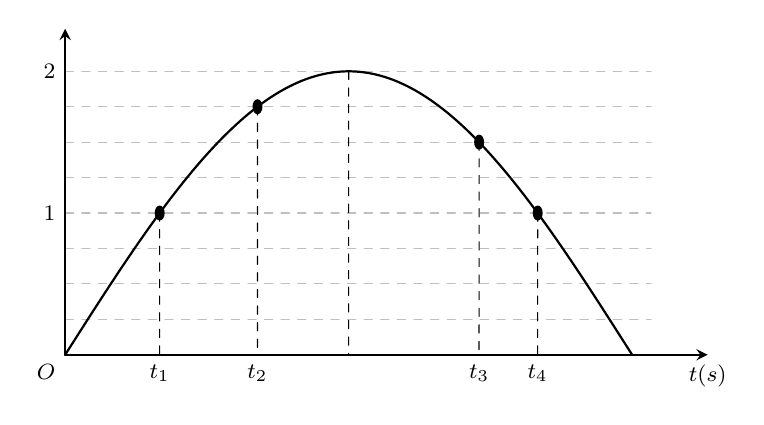
\begin{tikzpicture}[>=stealth, line join=round, line cap=round, font=\footnotesize, xscale=1.2, yscale=1.8]
		% Định nghĩa điểm
		\path (1, 1) coordinate (P1);
		\path (2.035, 1.75) coordinate (P2);
		\path (3, 2) coordinate (M);
		\path (4.38, 1.5) coordinate (P3);
		\path (5, 1) coordinate (P4);
		% Vẽ các đường phụ (đường lưới ngang)
		\foreach \i in {1,...,8} {
			\draw[dashed, gray!50, thin] (0, 0.25*\i) -- (6.2, 0.25*\i);
		}
		% Vẽ hệ trục tọa độ
		\draw[->, thick] (0, 0) -- (6.8, 0) node[below] {$t(\text{s})$};
		\draw[->, thick] (0, 0) -- (0, 2.3);
		% Vẽ đường cong đồ thị
		\draw[thick, domain=0:6, samples=150] plot (\x, {2*sin(\x*30)});
		% Vẽ các đường gióng dọc xuống trục hoành
		\draw[dashed] (P1) -- (1, 0);
		\draw[dashed] (P2) -- (2.035, 0);
		\draw[dashed] (M) -- (3, 0);
		\draw[dashed] (P3) -- (4.38, 0);
		\draw[dashed] (P4) -- (5, 0);
		% Nhãn trên các trục
		\node[below left] at (0, 0) {$O$};
		\node[left] at (0, 1) {$1$};
		\node[left] at (0, 2) {$2$};
		% Nhãn điểm và đánh dấu điểm bằng vòng lặp ở cuối
		\foreach \x/\l in {1/{t_1}, 2.035/{t_2}, 4.38/{t_3}, 5/{t_4}} {
			\node[below] at (\x, 0) {$\l$};
		}
		\foreach \p in {P1, P2, P3, P4} {
			\fill[black] (\p) circle (1.5pt);
		}
	\end{tikzpicture}
\end{center}
	\shortans[]{0,04}
	\loigiai{
		\begin{itemize}
			\item Trong quá trình dao động điều hòa bảo toàn năng lượng, động năng biến thiên liên tục đổi pha với thế năng. Lượng động năng cực đại đạt được khi đi qua vị trí cân bằng chính bằng giá trị cơ năng toàn phần của hệ:
			$$W_0 = W_{\text{đmax}} = 0,04\text{ J} \text{.}$$
		\end{itemize}
	}
\end{ex}

\Closesolutionfile{ans}

\noindent \textbf{PHẦN IV. Tự luận}
\vspace{0.2cm}

\begin{ex}%[11V1-2106-19]
	Một chiếc xe đẩy có khối lượng m được đặt trên hai bánh xe, mỗi bánh gắn một lò xo có cùng độ cứng $k = 200\text{ N/m}$. Xe chạy trên đường lát bê tông, cứ đi được quãng đường $6\text{ m}$ lại gặp một rãnh nhỏ ngăn cách. Với vận tốc tịnh tiến bằng $v = 14,4\text{ km/h}$ thì xe bị rung giật mạnh lắc dữ dội nhất. Lấy hằng số $\pi^{2} = 10$. Tính tổng khối lượng m của xe đẩy?
	\loigiai{
		\begin{itemize}
			\item Đổi đơn vị vận tốc tịnh tiến của xe sang mét trên giây: $v = 14,4\text{ km/h} = \frac{14,4}{3,6} = 4\text{ m/s}$.
			\item Khoảng thời gian định kì giữa hai lần liên tiếp bánh xe vấp phải rãnh nhỏ đóng vai trò là chu kì của ngoại lực cưỡng bức tác dụng kích thích:
			$$T_{\text{lực}} = \frac{s}{v} = \frac{6\text{ m}}{4\text{ m/s}} = 1,5\text{ s} \text{.}$$
			\item Xe bị rung lắc dữ dội mạnh nhất khi xảy ra hiện tượng cộng hưởng cơ vĩ mô, chu kì ngoại lực kích thích trùng khít với chu kì dao động riêng của hệ lò xo bánh xe đẩy:
			$$T_0 = T_{\text{lực}} = 1,5\text{ s} \text{.}$$
			\item Hệ hai bánh xe gắn song song hai lò xo cùng độ cứng tạo ra hệ lò xo tương đương có độ cứng tổng hợp bằng: $k_{\text{b}} = k_1 + k_2 = 200 + 200 = 400\text{ N/m}$.
			\item Hệ thức tính chu kì riêng của hệ khung xe đẩy:
			$$T_0 = 2\pi\sqrt{\frac{m}{k_{\text{b}}}} \Rightarrow T_0^2 = \frac{4\pi^2 m}{k_{\text{b}}} \Rightarrow (1,5)^2 = \frac{4 \cdot 10 \cdot m}{400}$$
			$$2,25 = \frac{40m}{400} \Rightarrow 2,25 = \frac{m}{10} \Rightarrow m = 22,5\text{ kg} \text{.}$$
		\end{itemize}
	}
\end{ex}

\begin{ex}%[11V1-2106-20]
	Cho đồ thị li độ theo thời gian của một vật dao động điều hoà có biên độ dải $A = 10\text{ cm}$, đường cong hình sin cắt trục hoành tại các mốc ô lưới chỉ ra chu kì dao động bằng $T = 4\text{ s}$. Xác định giá trị gia tốc của vật tại thời điểm sau $t = 2\text{ s}$ kể từ mốc ban đầu?
% TODO: \usepackage{graphicx} required
\begin{center}
	%\includegraphics[scale=1]{HINHVE-phai-Tikz/VL11-GHKI-PDL-2526-hinh11}
	\begin{tikzpicture}[xscale=1.3, yscale=0.18, >=Stealth]
		% Draw Axes
		\draw[->, thick] (-0.6, 0) -- (6.2, 0) node[right, yshift=0.1cm] {$t\text{ (s)}$};
		\draw[->, thick] (0, -12) -- (0, 13) node[above] {$x\text{ (cm)}$};
		% Origin
		\node[below left] at (0, 0) {$O$};
		% Dashed projection lines
		\draw[dashed, thin, gray] (0, 10) -- (4, 10);
		\draw[dashed, thin, gray] (4, 0) -- (4, 10);
		\draw[dashed, thin, gray] (0, -10) -- (2, -10);
		\draw[dashed, thin, gray] (2, 0) -- (2, -10);
		% Plot the harmonic wave: x = 10 * cos(pi/2 * t)
		\draw[very thick, blue!80!black, samples=300, domain=0:5.7] plot (\x, {10*cos(90*\x)});
		% Tick marks on t-axis
		\foreach \x in {1, 2, 3, 4, 5} {
			\draw (\x, 0.6) -- (\x, -0.6);
		}
		% Tick marks on x-axis
		\draw (0.05, 10) -- (-0.05, 10);
		\draw (0.05, -10) -- (-0.05, -10);
		% Labels
		\node[left, xshift=-0.05cm] at (0, 10) {$10$};
		\node[left, xshift=-0.05cm] at (0, -10) {$-10$};
		\node[below left, yshift=-0.05cm] at (1, 0) {$1$};
		\node[above, yshift=0.1cm] at (2, 0) {$2$};
		\node[above left, yshift=0.05cm] at (3, 0) {$3$};
		\node[below, yshift=-0.1cm] at (4, 0) {$4$};
		\node[above right, yshift=0.05cm] at (5, 0) {$5$};
		% Mark key points
		\foreach \p in {(0,10), (1,0), (2,-10), (3,0), (4,10), (5,0)} {
			\fill[red!80!black] \p circle (1.5pt);
		}
	\end{tikzpicture}
\end{center}
	\loigiai{
		\begin{itemize}
			\item Tần số góc dao động riêng của chất điểm: $\omega = \frac{2\pi}{T} = \frac{2\pi}{4} = 0,5\pi\text{ rad/s}$.
			\item Đổi đơn vị biên độ dài sang mét chuẩn: $A = 10\text{ cm} = 0,1\text{ m}$.
			\item Quan sát đồ thị hình sin đính kèm, tại thời điểm mốc thời gian $t = 2\text{ s}$ (bằng đúng một nửa chu kì $T/2$), đường cong đạt vị trí biên âm thấp nhất $\Rightarrow$ li độ của vật bấy giờ bằng $x = -A = -10\text{ cm} = -0,1\text{ m}$.
			\item Áp dụng công thức liên hệ động học tính giá trị gia tốc đại số của vật:
			$$a = -\omega^2 x = -(0,5\pi)^2 \cdot (-0,1) = 0,25\pi^2 \cdot 0,1 = 0,025\pi^2\text{ m/s}^2 \text{.}$$
			\item Nếu lấy hằng số xấp xỉ $\pi^2 \approx 10 \Rightarrow a \approx 0,025 \cdot 10 = 0,25\text{ m/s}^2$.
		\end{itemize}
	}
\end{ex}

\begin{ex}%[11V1-2106-21]
	Đồ thị hình vẽ bên mô tả sự thay đổi của thế năng đàn hồi $W_{\text{t}}$ theo li độ $x$ của quả cầu có khối lượng $m = 0,2\text{ kg}$ trong một con lắc lò xo treo thẳng đứng. Biết thềm biên giới hạn năng lượng cao nhất đạt $0,08\text{ J}$ tại vị trí vạch biên $x = 4\text{ cm}$. 
% TODO: \usepackage{graphicx} required
\begin{center}
	%\includegraphics[scale=1]{HINHVE-phai-Tikz/VL11-GHKI-PDL-2526-hinh12}
	\begin{tikzpicture}[>=stealth, line join=round, line cap=round, font=\footnotesize, scale=1.2]
		% Trục tọa độ
		\draw[->] (-3.2, 0) -- (3.2, 0) node[below] {$x$};
		\draw[->] (0, -0.5) -- (0, 3.8) node[right] {$W_t\text{ (mJ)}$};
		% Vẽ đồ thị (Parabol)
		\draw[thick, samples=100, domain=-2.5:2.5] plot (\x, {0.48*\x*\x});
		% Đường gióng nét đứt (vẽ theo chiều thuận kim đồng hồ)
		\draw[dashed] (-2.5, 0) -- (-2.5, 3.0) -- (2.5, 3.0) -- (2.5, 0);
		% Vạch chia trên trục hoành
		\draw[thick] (-2.5, -0.06) -- (-2.5, 0.06);
		\draw[thick] (2.5, -0.06) -- (2.5, 0.06);
		% Nhãn điểm
		\foreach \x/\y/\pos/\txt in {-2.5/0/below/-A, 2.5/0/below/A, 0/3.0/below right/40}
		\node[\pos] at (\x, \y) {$\txt$};
	\end{tikzpicture}
\end{center}
Xác định:
	\begin{enumerate}
		\item[a)] Cơ năng toàn phần của hệ con lắc lò xo.
		\item[b)] Giá trị thế năng của con lắc lò xo tại vị trí chất điểm đạt tốc độ chuyển động bằng $20\text{ cm/s}$.
	\end{enumerate}
		\loigiai{
			\begin{enumerate}
				\item[a)] Theo định luật bảo toàn năng lượng, giá trị thế năng đàn hồi đạt mức cực đại lớn nhất tại vị trí hai biên chính bằng cơ năng toàn phần của hệ dao động điều hòa:
				$$W = W_{\text{tmax}} = 0,08\text{ J} \text{.}$$
				\item[b)] Đổi đơn vị biên độ dài $A = 4\text{ cm} = 0,04\text{ m}$. Tính độ cứng $k$ của lò xo từ hệ thức cơ năng:
				$$W = \frac{1}{2}kA^2 \Rightarrow 0,08 = \frac{1}{2} \cdot k \cdot (0,04)^2 \Rightarrow 0,08 = 0,0008k \Rightarrow k = 100\text{ N/m} \text{.}$$
				\item Đổi tốc độ sang đơn vị m/s chuẩn hệ SI: $v = 20\text{ cm/s} = 0,2\text{ m/s}$.
				\item Động năng tức thời của quả cầu tại thời điểm tốc độ bằng $20\text{ cm/s}$ là:
				$$W_{\text{đ}} = \frac{1}{2}mv^2 = \frac{1}{2} \cdot 0,2 \cdot (0,2)^2 = 0,1 \cdot 0,04 = 0,004\text{ J} \text{.}$$
				\item Áp dụng hệ thức định luật bảo toàn tính thế năng tương ứng của hệ lò xo:
				$$W_{\text{t}} = W - W_{\text{đ}} = 0,08 - 0,004 = 0,076\text{ J} \text{.}$$
			\end{enumerate}
		}
	\end{ex}
	
	\Closesolutionfile{ans}
	
	\newpage
	%%%%%%%%%%%%%%%%%%%%%%%%%%%%%%%%%%%%%%%%%%%%%%%%%%%%%%%%%%%%%%%%%%%%%%%%%
	% KHUNG ĐÁP ÁN BẢNG TỰ ĐỘNG IN KẾT XUẤT CỦA HỆ THỐNG
	%%%%%%%%%%%%%%%%%%%%%%%%%%%%%%%%%%%%%%%%%%%%%%%%%%%%%%%%%%%%%%%%%%%%%%%%%
	\begin{center} \textbf{BẢNG ĐÁP ÁN THAM KHẢO MÃ ĐỀ THI 20} \end{center}
	
	\noindent \textbf{Phần I (Câu hỏi trắc nghiệm một phương án lựa chọn):}  
	\indapan{12}{ans/ansTN-PhanDangLuu2106}
	
	\noindent \textbf{Phần II (Câu hỏi trắc nghiệm Đúng/Sai):}
	\indapan[TF]{2}{ans/ansTF-PhanDangLuu2106}
	
	\noindent \textbf{Phần III (Câu hỏi trắc nghiệm trả lời ngắn):}
	\indapan[SA]{4}{ans/ansSA-PhanDangLuu2106}
	
	\label{B\thedeso}